\chapter{Background and Related Work}
\label{chapter:background}
This chapter outlines the history of the work done in the research area of forest fire modeling and simulation. It then gives some background information on GPU computation as well as the fuel models used by this research.

\section{Fire Models}
\subsection{Overview}
The most widely used fire model is that developed by Richard C. Rothermel. His model of fire spread model depicts fire spreading in an elliptical shape. Rothermel also developed the first eleven fuel models that are still used to this day \cite{roth}. A fuel model is a model of a small region of forest and the vegetation it contains. Examples of vegetation types that are modeled by the fuel models are grass and grass-dominated regions, chaparral and shrub fields, timber litter, and stash \cite{1983roth}. The method by which the first eleven fuel models were created is the basis for the development of all modern fuel models. The fuel model contains information on properties of the forest in a particular region, and at a certain granularity. The forest is broken up into cells, each cell having properties which are modeled in the fuel model. For example, one fuel model might describe a coniferous forest in regions of 30x30 meter cells. These cells are what make up the basis for a fire simulation. 

\subsection{Taxonomy of Fire}
There are three types of fire models: theoretical, empirical, and semi-empirical \cite{firereview}\cite{firereview2}. Empirical models use statistical descriptions of wildfires and do not attempt to include any real-world observations into their models. These models are mostly concerned with the shape of a fire. However, their lack of incorporation with physical data mean they are not as useful outside of controlled environments. Semi-empirical models incorporate some of the statistical modeling found in emperical models but also include experimentally derived approximations to portions of the models. Rothermel's spread equations are an important example of the semi-empirical fire models \cite{roth}. More detail on Rothermel's equations will follow in subsequent sections. The final type of models are theoretical, which rely solely on physical principles. Their limitation occurs at the boundary of what data is available. This work implements semi-emperical methods for calculating fire spread.

\subsection{Fire Shape}
The majority of the existing forest fire simulators, including this work, calculate wildfire spread based on the Rothermel's fire spread equations \cite{roth}. More detail on the simulators which use this fire spread model will be covered later in the section. Equation \ref{eq:roth} shows his rate of spread equation, which is based on several parameters. 

% \begin{equation}\sum_{i=0}^{\infty}x_i=\int_{0}^{\pi+2} f\end{equation}
\begin{equation} \label{eq:roth}
R = \frac{(I_{p})_{o}(1 + \phi_{w} + \phi_{s})}{\rho_{b}\varepsilon Q_{ig}}
\end{equation}

Where R is the rate of spread, $(I_p)_o$ is the no-wind propagating flux, $\phi_w$ and $\phi_s$ are the additional propagating flux introduced by wind and slope respectively. The product of $\rho_b$ and $\varepsilon$ is referred to as the effective bulk density. The effective bulk density models the amount of fuel per unit volume of the fuel bed raised to ignition ahead of the advancing fire. $Q_ig$ is the heat of preignition (the heat required to bring a unit weight of fuel to ignition). These values are derived from or contained in the fuel model that describes the cell for which the computations are being done. 

The desired output from a forest fire simulator is a time of arrival map. Each cell in this time of arrival map represents a cell in the simulation forest, and the value it contains is the time at which the cell ignited and started propagating the fire. Once a cell is lit, it begins contributing to the spread of the fire to the surrounding cells and continues burning until the fuel in that cell is entirely used. The method of propagation may vary between simulators, but the basic spread rate is usually based on Rothermel's equations.

\subsection{Surface Fire}
There are several potential approaches to calculating the propagation of the fire. This propagation also determines the method for stepping through time in a simulation. This work implemented three methods for iterating through a simulation to calculate the time of arrival map. The first two spread methods (Minimal Time and Iterative Minimal Time) are based on stepping through time independent of specific fuel conditions and are based on the paper by Sousa, dos Reis, and Pereira \cite{gpufire}. The third spread method implemented in this paper (Burn Distances) was based on code and methods found in vFire \cite{vFire}. 

vFire implemented an accurate spread rate calculator based on Rothermel's fire spread equations and the fire spread and fuel model data to propagate based upon the physical burning of fuel. The Burn Distances propagation method was based on their work.

Sousa, dos Reis, and Pereira also used the GPU to improve their running times and ported fireLib to the GPU \cite{gpufire}, but were the first to use the parallel programming language CUDA \cite{cuda}. They implemented three kernels in which they explored three different propagation types. The propagation methods labeled Minimal Time and Iterative Minimal time are based on their work. 

\begin{figure}%[!t]
\centering
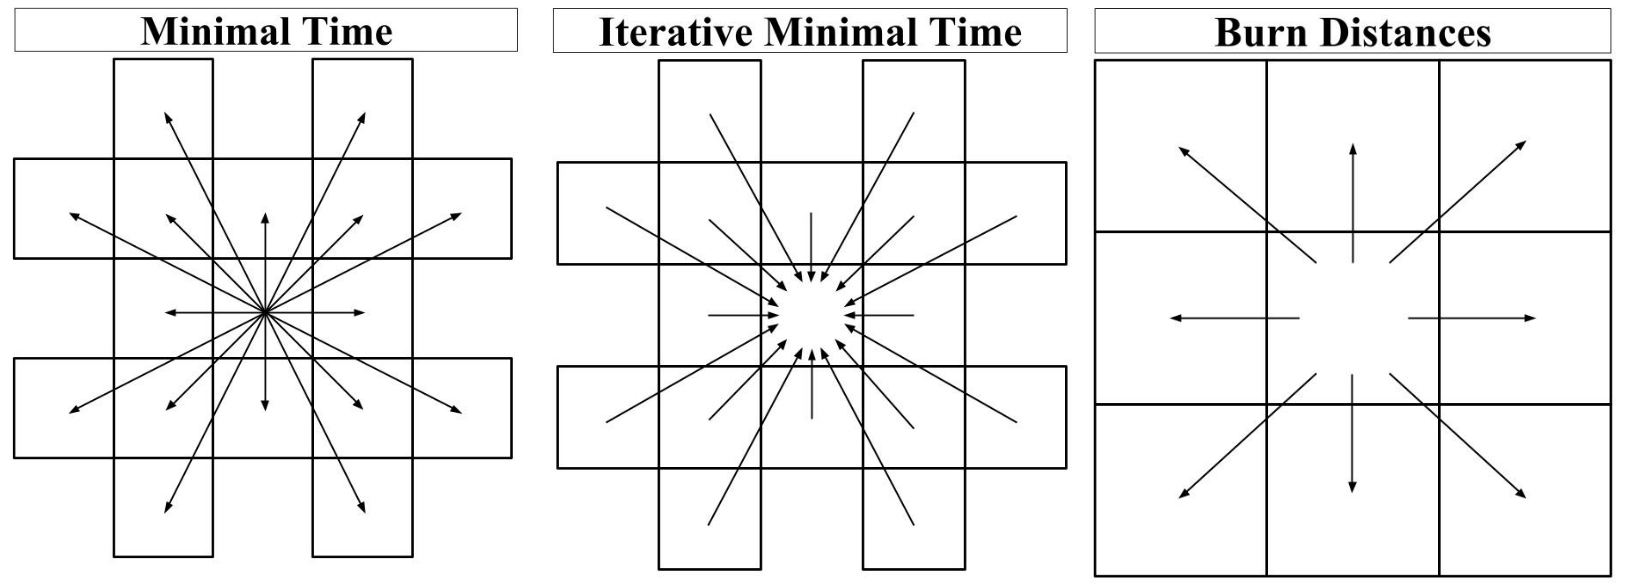
\includegraphics[width=\linewidth]{figures/background/spread_methods.PNG}
\caption{Neighbor access methodology for each of the propagation methods. From left to right: Minimal Time, Iterative Minimal Time, Burn Distances}
\label{fig:spreadTypes}
\end{figure}

\paragraph{Burn Distances}
The Burn Distances (BD) method is based on the idea that it takes a certain amount of time for fire to burn the distance between two cells. A distance is set as equivalent between all cells before the simulation burning may progress. The distance between cells is based on the properties of the forest model which is based on the size of the forest cell. The simulation iterates at a constant time step, and the amount the distance has burned is tracked throughout all the time steps. In this spread method, a cell looks to see which of its neighbors are on fire and which of those neighbors will burn the distance between the two cells first. The first cell to burn the total distance ignites the center cell as seen in Figure \ref{fig:spreadTypes}. In this work, the BD propagation method is based on work by Roger Hoang's vFire \cite{vFire}. The paper by Sousa, dos Reis, and Pereira also implemented a similar method, but it was not the basis for this propagation method in this work \cite{gpufire}.

\paragraph{Minimal Time}
The Minimal Time (MT) propagation method uses a dynamic time stepping method to step through the simulation. At each time step, a cell is examined to see if it is on fire. If the cell is burning, then the neighbors of the cell are examined as seen in Figure \ref{fig:spreadTypes}. If the neighbor is already on fire, it is ignored. If the neighbor is unlit, then the time of arrival for that cell is computed using the propagation equation found in Equation \ref{eq:rate}. In the Minimal Time method, time is incremented dynamically. Each time a new ignition happens, the ignition time is compared to the current 'timeNext' variable. If the new ignition time is smaller (the fire arrives sooner) than the current timeNext, then it replaces the timeNext value. This methodology means that time is incremented based on which cell will ignite the earliest. In the paper by Sousa, dos Reis, and Pereira, this method achieved the slowest speedup of their three methods \cite{gpufire}.

\paragraph{Iterative Minimal Time}
The Iterative Minimal Time (IMT) method is designed to avoid data dependencies. Each cell operates independent of its neighbors, calculating the ignition time based on the spread rates, and only finishing when the values between step $k$ and $k + 1$ converge. Each cell looks at the minimal time for each of its neighboring cells to burn towards it as shown in Figure \ref{fig:spreadTypes}. The value is known to converge after the difference between two time steps is less than some small threshold. The most appropriate value for this threshold can be determined through experimentation. In the work by Sousa, dos Reis, and Pereira, this method achieved the highest speedup of their three methods \cite{gpufire}. 

\subsection{Crowning}
Crowning is the phenomena of the fire moving from spreading along the base of the forest to up the trees to their crowns. There are two types of crowning: passive and active. A passive crown fire is one which does not spread to the overall propagation of the fire. Conversely, an active crown fire does contribute to the spread of the fire. The modeling method used for this implementation will be discussed in the Implementation section of this paper. The method for calculating crowning in this library was based on the work found in vFire \cite{vFire}. vFire based their implementation on the work found in FARSITE \cite{FARSITE}, which implemented their methods based on the work done by Van Wagner \cite{wagner1977}\cite{wagner1993}.

\subsection{Spotting}
Spotting occurs when firebrands from the wildfire are lifted into the air and fly ahead of the advancing flame wall to start new fires. There are three sequential components to spotting: generation, transport, and ignition. There are different models that describe the fire brand generation, and it depends on many factors such as degredation of wood due to pyrolisis and combustion. Research in this area consists of experiments that determine the behavior of burning wood, and generates data as to the size of potential brands \cite{firebrandgen}. Fire transport depends on many factors including flame structures, weather models, and the aerodynamics around the fire brand itself. There are several layers to the behavior of a fire brand before it reaches the open air: between the point of origin of the firebrand and the top of the flame, while the firebrand is between flame tip and buoyant plume, and when it is in the buoyant plume \cite{transport1}. The transport of the fire can be on a scale that is small, medium, or large \cite{transport2}. The ignition following the transport of the fire brand is dependent on the heat of the brand as it lands and the fuel properties it encounters \cite{firetecSpotting}. The studies that produce emperical data for igntion tests the success of a firebrand igniting a fire that successfully spreads a certain distance \cite{ignition}. The implementation found in this work does not go into great detail on the generation and ignition. The models have been extremely simplified to fit in the scope of this work. The generation is modeled simply at the point when Torching occurs. Torching is the event when a fire spreads from a base fire up into the tops of the trees as crowning occurs. Ignition is modeled as a simple user-defined probability. This method was implemented based on the work found in FARSITE \cite{FARSITE}. FARSITE based their implementation on the model developed by Albini in 1979 \cite{ablini}. The implementation found in this work had to be simplified somewhat because of constraints on the data available to the researchers. Details on the limitations found in spotting may be found in the Implmentation chapter of this paper. 

Another paper which implemented spotting did not use the same empirically-based methodology as the method used by FARSITE and in this paper. The work by Koo, Linn, Pagni, and Edminster implements a method for spotting based on the theoretical models known about physical phenomena surrounding wildfires \cite{firetecSpotting}. They experiment with different sized and shaped fire brands to determine the impact they have on the spotting distance possible during a forest fire. 

\section{Fire Simulators}
Since Rothermel's paper was published in 1972, several fire spread simulators have been developed. Nearly every major forest fire simulator has used his spread equations as the basis for their simulation. 

\subsection{BEHAVE}
The first major fire spread simulator was developed in 1986 called BEHAVE\cite{BEHAVE}. BEHAVE used Rothermel's fire propagation methods \cite{roth}. BEHAVE had two main functions to the application. The first function allowed users to load in fuel models from Rothermel's paper, but also to develop and save new fuel models. The simulator then had the ability to integrate the newly developed fuel models in its simulations. The second function of the application would run a simulation and burn prediction on the desired fuel model. The usefulness of the BEHAVE simulator is that it gives a realistic viewpoint of how a fire would behave given a specific fuel model at a specific instance in time. The output of this simulator appeared in a table which represented the times of arrival for each cell in the simulation. There was no visualization method available for this simulator. The simulation was meant to be used as a training tool rather than a real-time tool to be used to fight wildfires. It is still used to this day by fire scientists who are not familiar with the programming requirements of the newer simulators that have been developed. It remains a useful tool for fuel model development. 

\subsection{fireLib}
A decade later in 1996, BEHAVE was the basis for a new forest fire library that was developed using the programming language C called fireLib \cite{fireLib}. The code was based entirely on BEHAVE's simulator, but brought up to a then-modern platform. FireLib can run much faster than BEHAVE, and the output is given in time of arrival arrays rather than a table. Each [x,y] in the array corresponds to a cell in the fire simulation, and the time of arrival is the time at which the cell ignites, and can then begin to propagate the fire. The fire library is more flexible than BEHAVE and allows a user to design their own methods for propagating the fire. There are a few different methods which may be used, and will be addressed later in the paper. However, where BEHAVE was an entire application which had an interface component, fireLib is simply an open source forest fire library and both the visualization and interface development are left up to the user. fireLib incorporates the element of time that BEHAVE is missing, allowing researchers to look at a fluid time scale rather than a single instance of a fire. 

\subsection{FARSITE}
In 2004, FARSITE was developed, which works as a full-scale forest fire simulator \cite{FARSITE}. It has been continuously developed since 2004 and is currently still operational. It incorporates more features than simple fire spread, such as crown fires, surface fires, fire acceleration, and spotting. While it is one of the most advanced and accurate forest fire simulators, it is not very fast. The FARSITE simulator runs entirely sequentially, which it will be shown how slow a sequential implementation of these methods are later in this paper. Despite the lengthly amount of time required to compute its simulations, it is one of the most widely used forest fire simulators in existence today. A benefit of using FARSITE over other options is that they are able to incorporate advanced geospatial data.

\subsection{vFire}
This paper used much of the fire spread implemenation from a forest fire simulator called vFire \cite{vFire}. vFire was based on hFire, and are both cellular based spread models. They run faster than FARSITE, but do not have the same level of precision \cite{hFire}. vFire was the first forest fire simulator to utilize the parallel nature of the GPU to run calculations on the fire spread. At the time of its development, the only way to program on the GPU was to use the programming language OpenGL \cite{opengl}. vFire used the shader language glsl to utilize the multicore abilities of the GPU. vFire implemented a technique that has dynamic time stepping to burn distances between cells to determine an accurate time of arrival for the fire spread. The important feature that vFire accomplished was porting the computation of the fire spread to the GPU using OpenGL shaders \cite{opengl}. This simulator did not implement a sequential version to compare results against, and so there is no data to support how much improvement in runtime it accomplished. 

\subsection{FIRETEC}
Researchers at Los Alamos National Laboratory have created a fire simulator which is not based on the elliptical spread equations developed by Rothermel. Rather than using semi-empirical data to calculate their spread methods, they use theoretical models of chemical reactions and heat transfers to descipher where the fire is going to propagate \cite{firetech}. This method for calculating spread is very computationally expensive, and is used mainly for research purposes at the moment. 

\section{GPU Computation}
\subsection{Overview}
% History from CUDA site:
% http://www.nvidia.com/object/cuda_home_new.html
GPU's were originally designed as graphics accelerators supporting only very specific fixed-function pipelines. This meant that using them for high performance computation was not easy unless it could be integrated with some sort of visualization language. An example of such an integration may be seen in vFire \cite{vFire}. In 2006, NVIDIA released CUDA, which was the world's first solution to general-purpose computing on the GPU \cite{cuda}. Ever since its release, and even beforehand, the GPU was used for its high-processing capabilities. The architecture of the GPU allows for hundreds of low-powered processors to run in parallel. This type of computation is ideal for situations where the same computation to hundreds of inputs. The pitfalls of GPU computation occur when data dependencies exist in the data. If one portion of the data must wait on another to finish, it limits the usefulness of the GPU for processing. 

\subsection{CUDA}
CUDA is a parallel computing platform and computing model created by NVIDIA \cite{cuda}. It harnesses the hundreds of cores provided by a GPU an allows programmable kernels to be written. A kernel is a small bit of code that is run by a thread on the GPU. In the world of GPU programming, there is host data and device data. Host data is data which is stored on the home machine and processed by the CPU. Device data is data which is copied to the GPU for processing \cite{cudabyexample}. The architecture of a GPU that can be accessed through CUDA begins at the grid level. A single thread is assigned a thread ID. Each thread ID is unique among its block, which contains a certain number of threads. Many current GPUs have blocks that can contain up to 1024 threads. There may be many blocks in a single grid of a GPU, and the blocks may be assigned. The total number of threads would then be the number of blocks multiplied by the number of threads per block \cite{cuda}. An outline of the heterogeneous programming style may be seen in Figure \ref{fig:cuda_arch}. 

\begin{figure}%[!t]
\centering
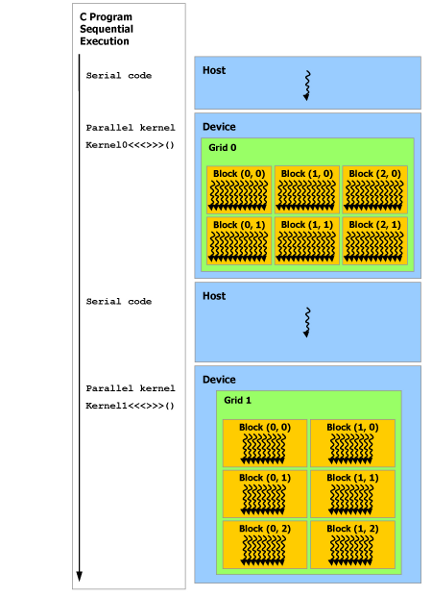
\includegraphics[height=7.5in]{figures/background/cuda_arch.png}
\caption{Outline of the programming style between the CPU and GPU \cite{cuda}.}
\label{fig:cuda_arch}
\end{figure}

In order to test the work presented in this paper, the tests were run on a CUBIX box \cite{cubix}. The CUBIX box is designed to leverage multi-GPU and CPU programming. The box contains seven GPUs and four CPUs. This work only implements single-GPU simulations. The reason the CUBIX box was used was for the speed of determining results. It allows several simulations to be run and timed simultaneously, which meant the results could be gathered faster. 

\section{Fuel Models}
The data needed to process the fire simulation begins with the Fuel Models required by the simulator. Rothermel developed thirteen original fuel models, which are still used today \cite{1983roth}. Additional fuel models have been developed since that time, 42 of which are incorporated into this work. Additional fuel models, including those of what are called 'unburnable' in this work may be found in the work by Scott and Burgan \cite{fuelmodels}.  The fuel models contain data regarding surface-area-to-volume ratio by class and component, fuel model type, fuelbed depth, extinction moisture content, and fuel particle heat content. These data types are used to determine the behavior of the fire in a particular cell of the simulation. The details on the data available may be found in the documentation of the library. 